% Created 2017-04-19 Wed 09:15
\documentclass[11pt]{article}
\usepackage[utf8]{inputenc}
\usepackage[T1]{fontenc}
\usepackage{fixltx2e}
\usepackage{graphicx}
\usepackage{longtable}
\usepackage{float}
\usepackage{wrapfig}
\usepackage{rotating}
\usepackage[normalem]{ulem}
\usepackage{amsmath}
\usepackage{textcomp}
\usepackage{marvosym}
\usepackage{wasysym}
\usepackage{amssymb}
\usepackage{hyperref}
\tolerance=1000
\date{April 17-21, 2017}
\title{Week 13 lecture notes - PSYC 3435}
\hypersetup{
  pdfkeywords={},
  pdfsubject={},
  pdfcreator={Emacs 25.1.1 (Org mode 8.2.10)}}
\begin{document}

\maketitle
This week we will finish talking about nonexperimental designs with two new types of designs: \emph{developmental designs} and \emph{small N designs}

\section*{Developmental designs}
\label{sec-1}

Used to study changes in behavior that occur as a function of \emph{changes in age}
\begin{itemize}
\item age = quasi-independent variable
\end{itemize}

Three major types:
\begin{itemize}
\item cross-sectional
\item longitudinal
\item cohort-sequential
\end{itemize}

\subsection*{Cross-sectional design}
\label{sec-1-1}
\begin{itemize}
\item study groups of individuals of different ages at the same time
\item age is treated as a \emph{between-subjects} variable
\end{itemize}

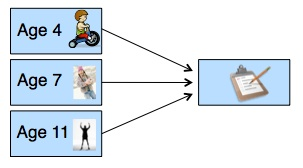
\includegraphics[width=.9\linewidth]{figures/crossSectional.jpg}

Advantages:
\begin{itemize}
\item much faster -- can gather data about different groups (ages) at the same time
\end{itemize}

Disadvantages:
\begin{itemize}
\item individuals not followed over time (does not reveal \emph{development} of individuals)
\item cohort effects: individuals of different ages may be inherently different due to factors in the environment
\end{itemize}

\subsection*{Longitudinal design}
\label{sec-1-2}
\begin{itemize}
\item study same invididuals/groups over time
\item age is treated as a \emph{within-subjects} variable
\end{itemize}

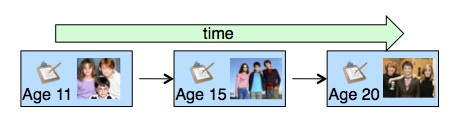
\includegraphics[width=.9\linewidth]{figures/long.jpg}

Advantages:
\begin{itemize}
\item can see developmental changes
\item avoid cohort effects
\end{itemize}

Disadvantages:
\begin{itemize}
\item time consuming
\item attrition and practice effects
\end{itemize}

\subsection*{Cohort-sequential design}
\label{sec-1-3}
\begin{itemize}
\item measure groups of participants as they age
\item combines best parts of cross-sectional and longitudinal designs
\end{itemize}

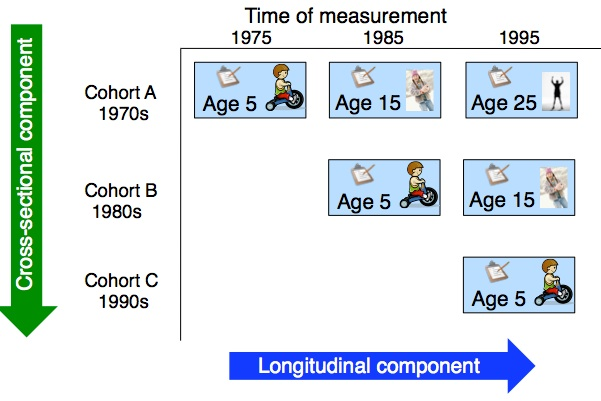
\includegraphics[width=.9\linewidth]{figures/seq.jpg}

\section*{Small $N$ designs}
\label{sec-2}

Used to study behavior is a small number of participants.

Two main types:
\begin{itemize}
\item Discrete trials design
\begin{itemize}
\item large number of trials completed by small number of participants
\item used to study basic behavioral processes that are not likely to differ between people (e.g., learning, attention, memory, etc.)
\item ex: Ebbinghaus studies -- one participants, MANY trials
\end{itemize}

\item Baseline designs
\begin{itemize}
\item observations begin at \emph{baseline} (absence of a treatment)
\item Basic idea: you want to show that
\begin{itemize}
\item when treatment occurs, you get an effect
\item when you remove the treatment, the effect reverses
\end{itemize}
\end{itemize}
\end{itemize}

Most common example: ABA design

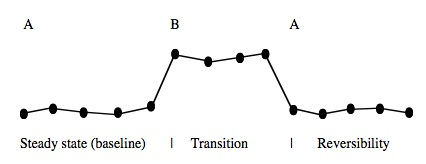
\includegraphics[width=.9\linewidth]{figures/aba.jpg}
% Emacs 25.1.1 (Org mode 8.2.10)
\end{document}